\section{Modeling}
\label{method}
In this section, we present the modeling strategies of \textbf{MiniOneRec}, as illustrated in Figure \ref{fig:framework}. 
MiniOneRec first converts the textual information into SIDs with the RQ-VAE tokenizer (Section \ref{sec:tokenization}). 
For better incorporating the huge world knowledge within LLMs \citep{LlaRA}, MiniOneRec further introduces the alignment with LLMs as one expansion of the original OneRec architecture (Section \ref{sec:alignment_llm}). 
During the training stage, MiniOneRec is optimized with next token prediction first, and then followed by reinforeced preference optimization (Section \ref{sec:optimization}). 


\begin{figure}
    \centering
    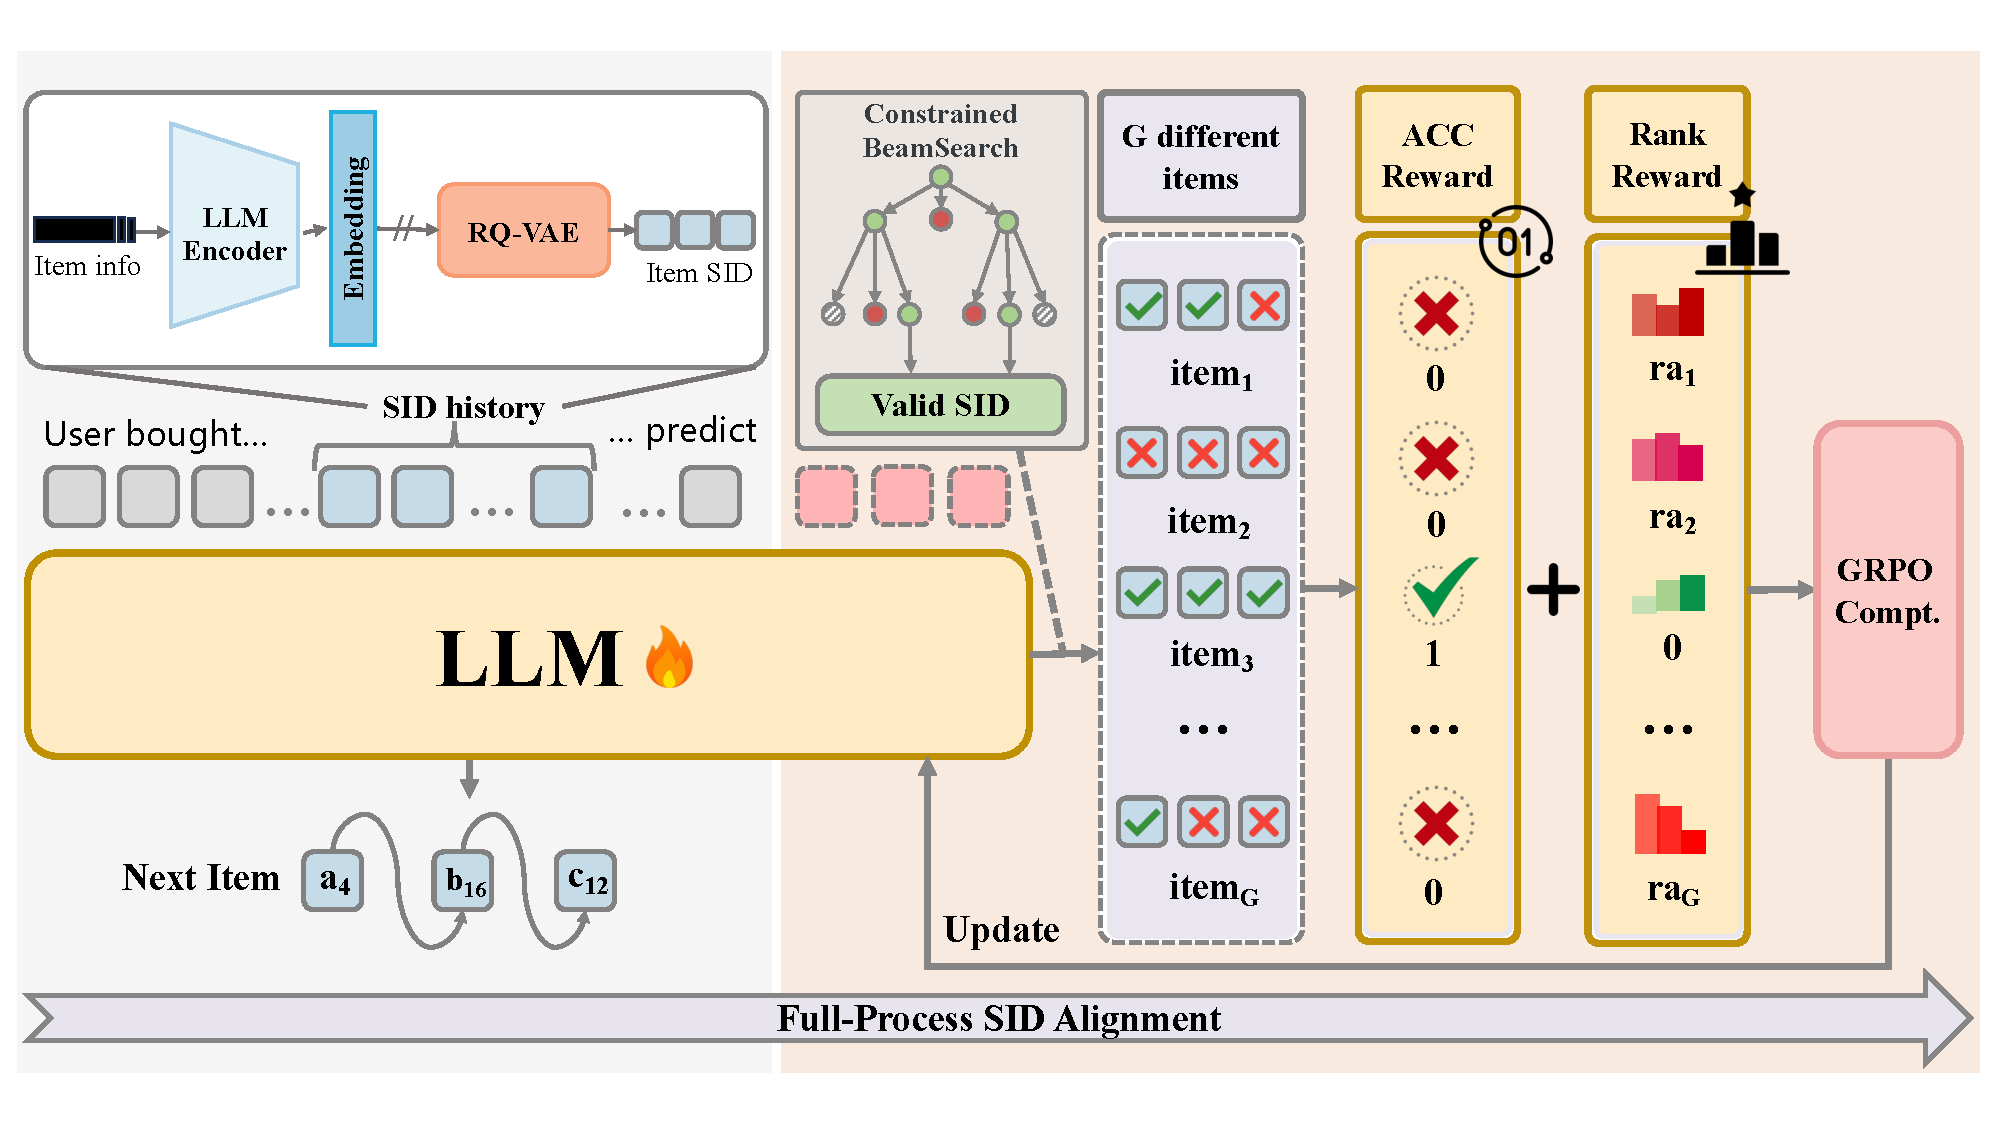
\includegraphics[width=0.85\textwidth]{figures/MiniOneRec_framework.pdf}
    \vspace{-10pt}
    \caption{MiniOneRec framework. RQ-VAE builds the item SID codebook. We then perform SFT to warm up the LLM and obtain an initial alignment. In RL, beam search with constrained decoding, thereby the model sequentially produces a ranked list of distinct, valid SIDs. GRPO updates the policy, and SID alignment is enforced end-to-end. This alignment objective is preserved throughout both the SFT and RL stages, fostering deeper semantic understanding.}
    \label{fig:framework}
    \vspace{-10pt}
\end{figure}

% To address the key shortcomings of the existing SFT-then-RL pipeline for generative recommendation, we propose \textbf{MiniOneRec}.  
% The framework elevates the performance ceiling by aligning the LLM with the SID space throughout the entire training process and applying preference optimization in the RL stage, as illustrated in Figure \ref{fig:framework}.

\subsection{Task formulation}

We first formulate recommendation as a sequence–generation problem.  
For every user $u$, the items he or she has interacted with are sorted chronologically to form a sequence
$H_u=\bigl[i_1,i_2,\dots,i_T\bigr]$.  
Each item $i_t$ in the sequence is encoded by a three–level structural ID, $\bigl\{c_0^{i_t},\,c_1^{i_t},\,c_2^{i_t}\bigr\}$. Such structural IDs are typically called SIDs, which preserve hierarchical semantics through quantization techniques with semantic embeddings \citep{TIGER}.
% since they are 
% so that hierarchical semantics are preserved.

A generative policy $\pi_\theta$, implemented as an autoregressive model with parameters $\theta$, reads the entire history $H_u$ and is trained to predict the next item $i^{+}$ that best matches the taste of user $u$ among all candidates in the catalog.  
During inference, the model recursively produces item tokens; we keep the $k$ most promising beams by the standard beam–search algorithm and return them as the recommendation list.  
Model performance is reported with the evaluation measures commonly adopted in generative recommendation.


\subsection{Item Tokenization} \label{sec:tokenization}

In SID-style generative recommenders, the first task is to convert each item into a sequence of discrete tokens. Following the practices of TIGER \citep{TIGER}, we employ RQ-VAE~\citep{rqvae} for this purpose. % The procedure is as follows: (1) For every item $i$, we concatenate its title and textual description to form a single sentence; (2) This sentence is passed through a frozen text encoder \citep{AlphaRec}, producing a $d$-dimensional semantic vector $\mathbf{x}\in\mathbb{R}^{d}$; (3) RQ-VAE then applies multi-stage residual quantization to $\mathbf{x}$, gradually approximating it and finally yielding a list of discrete codewords. These codewords are used as the item representation in the subsequent generative recommendation module.
Concretely, the pipeline is:

\begin{enumerate}
    \item For every item $i$, we concatenate its title and textual description to form a single sentence;  
    \item This sentence is passed through a frozen text encoder \citep{AlphaRec}, producing a $d$-dimensional semantic vector $\mathbf{x}\in\mathbb{R}^{d}$;  
    \item Apply RQ-VAE to $\mathbf{x}$. At each level $l$ ($0\le l<L$) we have a separate codebook $\mathcal{C}_l=\{\mathbf{e}^{(l)}_{k}\}_{k=1}^{K}$, where $K$ is the codebook size. We set $L{=}3$ and $K{=}256$, so each item is represented by three bytes; this choice provides $2^{24}$ possible codes, which is sufficient for catalogs containing hundreds of millions of products while keeping the vocabulary small. The residual is initialized as $\mathbf{r}_{0}=\mathbf{x}$ and updated by
    \[
       c_l=\arg\min_{k}\left\|\mathbf{r}_l-\mathbf{e}^{(l)}_{k}\right\|_2,\qquad 
       \mathbf{r}_{l+1}=\mathbf{r}_l-\mathbf{e}^{(l)}_{c_{l}}.
    \]
    \item Collect the indices $(c_0,\dots,c_{L-1})$ as the discrete token sequence for item $i$; these indices constitute the item tokens consumed by the subsequent generative recommender.
\end{enumerate}

The quantized latent is reconstructed by
\[
    \mathbf{z}_{\text{q}}=\sum_{l=0}^{L-1}\mathbf{e}^{(l)}_{c_l},
\qquad
    \hat{\mathbf{x}}=D(\mathbf{z}_{\text{q}}),
\]
where $D(\cdot)$ is a decoder. The codebooks, the encoder and the decoder are trained jointly, while the text encoder remains frozen. The loss is the sum of a reconstruction term and an RQ regularizer:
\[
\mathcal{L}(\mathbf{x})=
\underbrace{\left\|\mathbf{x}-\hat{\mathbf{x}}\right\|_2^{2}}_{\mathcal{L}_{\text{RECO}}}
+\underbrace{\sum_{l=0}^{L-1}\!\bigl(
      \|\mathrm{sg}[\mathbf{r}_l]-\mathbf{e}^{(l)}_{c_l}\|_2^{2}
      +\beta\,\|\mathbf{r}_l-\mathrm{sg}[\mathbf{e}^{(l)}_{c_l}]\|_2^{2}\bigr)}_{\mathcal{L}_{\text{RQ}}},
\]
with $\mathrm{sg}[\cdot]$ the stop-gradient operator and $\beta$ a hyper-parameter controlling the commitment term.

To prevent codebook collapse, we follow the warm-start trick in prior work \citep{rqvae, LCRec} and initialize each codebook with $k$-means centroids computed on the first training batch.


\subsection{Alignment with LLMs} \label{sec:alignment_llm}
LLMs possess extensive understanding of the world and human behaviors 
\citep{AlphaRec}, which can serve as a supplement to the collaborative signals in recommender systems \citep{RLMRec}.
Existing work has shown that linking an LLM’s world knowledge to SID representations noticeably strengthens generative recommendation \citep{LlaRA, LCRec}. Therefore, rather than training on SIDs alone as in prior work \citep{TIGER, OneRec, mtgr}, we introduce several alignment objectives that tie the language space to SID signals. Two major groups of tasks are employed:  
\begin{itemize}
    \item \textbf{Recommendation Tasks}: The LLM receives a time-ordered history together with a clear instruction and is asked to predict the SID of the next item the user might engage with.  
    \item \textbf{Alignment Tasks}: A collection of bridging tasks enforces a two-way mapping between natural language and SID space, grounding the discrete codes in text while injecting linguistic knowledge into their embeddings.  
\end{itemize}
Tasks from both groups are optimized jointly throughout the SFT stage and the subsequent RL stage. During RL, we adopt constrained decoding so that the model can only produce tokens from a predefined list containing every item’s SID and its canonical title. This constraint guarantees valid outputs and enables straightforward, rule-based reward computation. Detailed examples of the prompts are provided in the Appendix \ref{appendix:align_prompt}.


\subsection{Reinforced Preference Optimization} \label{sec:optimization}
After SFT, we further polish the policy with GRPO~\citep{deepseekmath,deepseek}. GRPO differs from classic RLHF in that it draws multiple candidates per prompt and normalizes rewards within the group, which reduces gradient variance.

Steps:
(1) For every prompt $x\!\sim\!D$, the frozen policy $\pi_{\theta_{\text{old}}}$ is rolled out $G$ times, yielding $\mathcal{Y}(x)=\{y^{(1)},\ldots,y^{(G)}\}$.  
(2) Each candidate $y^{(i)}$ is assigned a scalar score $S_i$.  
(3) Advantages are standardized inside the group:
\[
\hat{A}_i=\frac{S_i-\mu_{1:G}}{\sigma_{1:G}},
\]
where $\mu_{1:G}$ and $\sigma_{1:G}$ denote the mean and standard deviation of the $G$ rewards.

The surrogate objective becomes
\[
\small
\begin{aligned}
J_{\text{GRPO}}(\theta)=
\mathbb{E}_{x,y^{(i)}}
\biggl[
\frac{1}{G}\sum_{i=1}^{G}\frac{1}{|y^{(i)}|}
\sum_{t=1}^{|y^{(i)}|}
\!\Bigl(
\min\!\bigl(w_{i,t}\hat{A}_{i,t},\,
\operatorname{clip}(w_{i,t},1-\epsilon,1+\epsilon)\hat{A}_{i,t}\bigr)
-\beta\,\mathrm{KL}\!\bigl[\pi_\theta\|\pi_{\text{ref}}\bigr]
\Bigr)
\biggr],
\end{aligned}
\]
with token-level importance ratio  
$w_{i,t}= \dfrac{\pi_\theta(y^{(i)}_t\!\mid\!x,y^{(i)}_{<t})}
                 {\pi_{\theta_{\text{old}}}(y^{(i)}_t\!\mid\!x,y^{(i)}_{<t})}$.
The parameter $\epsilon$ controls clipping, while $\beta$ keeps the updated policy near a reference model through a KL term.


Applying RL with verifiable rewards (RLVR) to recommendation brings two obstacles:

\begin{itemize}
    \item \textbf{Unique generation space}. The action space is a closed set of item SIDs, orders of magnitude smaller than natural-language vocabularies. Re-sampling tends to produce duplicates, wasting computation. We therefore mix dynamic sampling \citep{DAPO} with constrained beam search to enlarge coverage while keeping outputs valid.
    \item \textbf{Sparse ranking supervision}. A hard binary reward (1 for the correct item, 0 otherwise) offers little guidance on ranking quality. We introduce an auxiliary ranking-shaped reward to penalize harder negatives with lower scores. Additionally, dense signals such as semantic similarity and collaborative scores are explored to furnish richer supervision.
\end{itemize}
\subsubsection{Sampling Strategy}
\label{subsection:sampling}

A practical obstacle when porting RLVR to recommendation is the poor sampling diversity brought by the limited action space: querying the policy multiple times with the same prompt often returns identical items, so the model observes few distinct negatives. We measure diversity via
\[
\mathrm{Div}\!\left(\{e_k\}_{k=1}^G\right)=
\frac{\bigl|\text{Unique}\bigl(\{e_k\}_{1}^{G}\bigr)\bigr|}{G},
\]
where the numerator counts unique items among the $G$ generations. Higher values indicate richer supervision.

Two complementary remedies are investigated:

\begin{itemize}
    \item \textbf{Dynamic Sampling} \citep{DAPO}. We first over-sample, then pick a subset that (i) must include the ground-truth item and (ii) maximizes internal diversity. Although helpful, this demands extra forward passes and still deteriorates as training progresses.

    \item \textbf{Beam Search}. We ultimately switch to beam search without length normalization \citep{D3, ReRe}. By construction, all beams differ, so the method guarantees zero duplication within each group and yields better diversity–efficiency trade-offs.
\end{itemize}

Based on our findings, MiniOneRec ultimately employs constrained beam search as its default sampler, ensuring that every generated item is valid while still providing a diverse set of candidate trajectories.

\subsubsection{Reward Design}
\label{method:reward}

Recommendation models are usually judged with ranking measures such as NDCG. In contrast, the standard GRPO setup supplies a binary reward, giving a value of $1$ to the true item and $0$ to every other candidate. This strategy treats all negatives as equally harmful. Earlier studies \citep{SGL,sdpo} have shown that focusing on hard negatives produces stronger rankers. Motivated by these results, we introduce a rank-aware reward that assigns different penalties based on how prominently a negative item appears in the model’s own ranking \citep{ReRe}.

Given a negative candidate $e_k$ whose generation probability ranks $\rho_k$ (with $\rho=1$ the most probable), we set
\[
\tilde{R}_{\text{rank}}(e_k,e_t)=
\begin{cases}
0, & e_k=e_t,\\
-\dfrac{1}{\log(\rho_k+1)}, & \text{otherwise},
\end{cases}\;\;
R_{\text{rank}}(e_k,e_t)=
-\dfrac{\tilde{R}_{\text{rank}}(e_k,e_t)}
{\sum_{j=1}^{G}\tilde{R}_{\text{rank}}(e_j,e_t)}.
\]
Thus, negatives that the model was very confident about (low $\rho_k$) receive stronger penalties.

The final reward combines rule-based and ranking components:
\[
R(e_k,e_t)=R_{\text{rule}}(e_k,e_t)+R_{\text{rank}}(e_k,e_t),
\]
where the rule-based term is
\[
R_{\text{rule}}(e_k,e_t)=
\begin{cases}
1, & e_k = e_t,\\
0, & \text{otherwise}.
\end{cases}
\]
The mixed reward discussed combines binary correctness with a soft ranking term, helping the LLM tell hard negatives apart. Yet recommendation data contain additional, under-utilized cues. To see whether such information can enhance or even replace the rule-based component in RLVR, we experiment with the following collaborative reward. Specifically, for every item suggested by the policy, we obtain its logit from a pre-trained collaborative-filtering model and pass that score back as reward, thereby injecting knowledge extracted from historical user–item interactions. MiniOneRec ultimately adopts the combined ranking-and-rule reward as its default choice.



